%%%%%%%%%%%%%%%%%%%%%%%%%%%%%%%%%%%%%%%%%%%%%%%%%%%%%%%%%%%%%%%%%%%%%%%%%%%%%%%%
%2345678901234567890123456789012345678901234567890123456789012345678901234567890
%        1         2         3         4         5         6         7         8

\documentclass[letterpaper, 10pt, conference]{ieeeconf}

\IEEEoverridecommandlockouts
\usepackage{cite}
\usepackage{url}
\overrideIEEEmargins
\usepackage{textcomp}
\usepackage{gensymb}
\usepackage{graphicx}
\usepackage{array}
\usepackage{amsmath}
\usepackage{amssymb}
\usepackage[utf8]{inputenc}
\usepackage{booktabs}

\begin{document}

\title{Experience: Evidence-Aware Pre-Execution Plan Assessment for Generative Robotic Behaviour Planning}

% \author{Kalana Ratnayake$^{1}$, Michael Pritchard$^{2}$, Maleen Jayasuriya$^{3}$, Damith Herath$^{4}$%
% \thanks{$^{1}$Kalana Ratnayake is with Collaborative Robotics Laboratory, Faculty of Science and Technology, University of Canberra, ACT, Australia {\tt\small Kalana.Ratnayakemudiyanselage@canberra.edu.au}}%
% \thanks{$^{2}$Michael Pritchard is with Collaborative Robotics Laboratory, Faculty of Science and Technology, University of Canberra, ACT, Australia {\tt\small Michael.Pritchard@canberra.edu.au}}%
% \thanks{$^{3}$Maleen Jayasuriya is with Collaborative Robotics Laboratory, Faculty of Science and Technology, University of Canberra, ACT, Australia {\tt\small Maleen.Jayasuriya@canberra.edu.au}}%
% \thanks{$^{4}$Damith Herath is with Collaborative Robotics Laboratory, Faculty of Science and Technology, University of Canberra, ACT, Australia {\tt\small Damith.Herath@canberra.edu.au}}%
% }

\maketitle

\begin{abstract}
Generative robotic behaviour planning can produce plausible behaviour plans from a composition of elementary robot behaviours to satisfy natural-language tasks, but these systems tend to treat generated plans as equally executable until failure occurs at runtime. This is a weakness for deployed robots, because a plan may be semantically valid while still being slow, fragile, poorly grounded in available evidence, or mismatched to the robot's state. We introduce \textit{Experience}, a plan audit layer that sits between behaviour discovery and execution and performs pre-execution plan assessment to rank semantically valid compositional behaviour plans. Experience combines a semantic graph for behaviour and task meaning with a statistical graph for empirical execution evidence, then ranks candidate plans with a Risk-Aware Plan Feasibility Score (RAPFS) that focuses on predicted success, time, energy, fault burden, resource considerations, and epistemic uncertainty. We utilise \textit{Fabric} as a generative behaviour planning system and extend its functionality using the proposed \textit{Experience} layer. We compare the standalone \textit{Fabric} planner against the \textit{Experience-augmented Fabric} planner to evaluate whether evidence-aware pre-execution assessment improves candidate plan selection.
\end{abstract}

\begin{keywords}
robot planning, pre-execution verification, ROS2, risk-aware planning, knowledge graphs, uncertainty-aware ranking
\end{keywords}

\section{Introduction}

Autonomous robots operating in dynamic environments require planning systems that can do more than produce a single behavioural policy. Sequences of actions are composed of distinct, plausible and repeatable elementary behaviours to create complex behaviours for real-world environments. State-of-the-art behaviour-based planning systems provide methods for designing composite behaviours \cite{ghzouli_behavior_2023}. A composed plan that looks reasonable when designed may still be a poor operational choice when the robot is low on battery, when a required behaviour has recently failed, when a dependency chain is poorly observed, or when the current scene differs from the contexts under which the robot has previously succeeded. This distinction matters more in long-horizon and open-ended tasks, where the cost of discovering infeasibility only after execution has begun can be high in time, energy, and recovery effort.

One approach to accounting for longer horizons and open-endedness is to generate new plans during operation. Recent progress in large language models has made \textit{generative} behaviour-based robot planning substantially more feasible. SayCan showed that language-model planning improves when abstract task semantics are grounded in executable robot skills rather than treated as free-form text \cite{ahn_as_2022}. SayPlan extended this idea to larger environments by using 3D scene graphs, semantic retrieval, and iterative replanning for long-horizon tasks \cite{rana_sayplan_2023}. Behaviour-tree-based systems such as BTGenBot, LLM-BT, and LLM-as-BT-Planner further improved the planning surface by generating structured intermediate plans that are easier to inspect and execute than raw code \cite{izzo_btgenbot_2024, zhou_llm-bt_2024, ao_llm-as-bt-planner_2025}. \cite{ratnayake2026generativepartiallyspecifiedfinite} contributes to this line of work by providing \textit{Fabric}, a graph-based generative behaviour planning framework built around partially specified finite-state machines and the Capabilities2 execution layer.

However, most generative planning pipelines still prioritise generation over assessment. They typically retrieve behaviour descriptions, context, and occasionally telemetry to support prompt construction, but they rarely impose a distinct pre-execution stage that evaluates candidate plans against accumulated evidence of how those behaviours perform under similar conditions. As a result, the planner may select a semantically valid plan when historical evidence suggests that the behaviour or combination is unreliable, overly costly, or weakly supported by prior observations. In practical deployment this means that plan feasibility is only tested through live execution where failures are costly to recover from.

This paper argues that pre-execution plan assessment should be treated as its own planning layer. We propose that this layer should combine two distinct forms of knowledge. The first is semantic structure, which captures what a behaviour means, what it does, how it can be composed, and how it relates to the task. The second is empirical evidence, which captures how those behaviours have actually performed at runtime. These roles should remain separate because semantic similarity is not equivalent to execution reliability. A behaviour can be an excellent semantic match for a request and still be a poor execution choice if it is slow, failure-prone, or poorly observed in the current context.

We implement this idea through the \textit{Experience} layer, a ROS2 planning extension that sits between behaviour discovery and execution. Experience uses Capabilities2 \cite{pritchard_capabilities2_2025, woodall_ros_2014} as the behaviour description and orchestration layer, consumes candidate plans produced for \textit{Fabric} \cite{ratnayake2026generativepartiallyspecifiedfinite}, and ingests runtime evidence from the \textit{Supervisor} subsystem. In this way, experience is not a replacement for generative planning; it is an evidence-aware assessment layer that ranks candidate behaviour execution graphs before one is selected and dispatched.

The main contributions of this paper are threefold. First, we define a dual-graph knowledge representation consisting of linked semantic and statistical graphs for behaviour-centric robotic planning. Second, we formulate a Risk-Aware Plan Feasibility Score (RAPFS) that ranks candidate behaviour plans using predicted success, execution cost, fault burden, and epistemic uncertainty under explicit feasibility constraints. Third, we present a ROS2 implementation built around \textit{Fabric}, \textit{Capabilities2}, \textit{Experience}, and \textit{Supervisor}, and use it to frame an experimental comparison between direct generative planning and evidence-aware pre-execution plan assessment.

\section{Related Work}

Generative robot planning has progressively shifted from direct action selection to code generation, then towards structured intermediate representation composition. SayCan grounded language-model suggestions in pretrained robot skills and their affordance values, showing that embodied skill grounding improves long-horizon task execution \cite{ahn_as_2022}. SayPlan extended this idea with hierarchical 3D scene-graph retrieval and iterative replanning, making LLM-based planning more scalable in larger environments \cite{rana_sayplan_2023}. ROS-LLM similarly framed LLM-assisted robot programming around structured reasoning, task feedback, and multiple execution modes, including sequences, behaviour trees, and state machines \cite{mower_ros-llm_2024}. These systems reduce purely textual hallucination, but they remain primarily generation-oriented. They help construct or adapt plans; they do not provide a general evidence-aware scoring layer that compares multiple candidate execution graphs before dispatch.

Behaviour-tree-based generation has become the most visible structured alternative to direct code output. BTGenBot fine-tunes lightweight local LLMs for BT generation and evaluates the resulting trees with syntax checks, a validation system, simulation, and real robot trials \cite{izzo_btgenbot_2024}. LLM-BT focuses on adaptive task execution by converting LLM-generated task steps into behaviour trees and updating those trees when environmental changes are detected \cite{zhou_llm-bt_2024}. LLM-as-BT-Planner presents a more complete generation-to-execution pipeline for behaviour-tree planning \cite{ao_llm-as-bt-planner_2025}, while VLM-driven BT extends the same idea to visual conditions so generated trees can react to image-grounded state checks \cite{wake_vlm-driven_2025}. These papers align strongly with the present work because they all move planning toward inspectable symbolic structures. Their common limitation for our purpose is not representational validity but lack of a distinct pre-execution ranking stage that uses accumulated execution evidence to prefer one valid candidate over another.

There is also a smaller but relevant line of work around execution representations and planning surfaces. The broader BT and FSM literature has repeatedly shown that representation choice affects modularity, reuse, and verification effort \cite{ghzouli_behavior_2023, iovino_programming_2022, iovino_comparison_2024}. The authors of the GPSFSM \cite{ratnayake2026generativepartiallyspecifiedfinite} argue that \textit{partially specified} finite-state-machine semantics provide a more general execution graph than tree-only control structures for generative planning. \textit{Experience} does not replace that representation; rather, it assumes the planner can already produce candidate execution graphs and addresses the next question, namely which candidate should be executed given current evidence.

At the capability layer, the original ROS capabilities package and Capabilities2 solve a different but necessary problem: how robot behaviours are described, loaded, related, and executed in a standard form \cite{woodall_ros_2014, pritchard_capabilities2_2025}. Capabilities2 is especially relevant because it provides a structured, ROS2-native description of behaviour interfaces and providers that can be queried at runtime. This makes it a stronger substrate for evidence-aware planning than ad hoc prompt-only capability descriptions. Experience builds directly on this layer, but Capabilities2 itself is not a plan-generation or plan-selection framework; it describes what the robot can do, not which candidate plan is most feasible.

The question of reliability has recently been revisited through uncertainty estimation. CURE explicitly separates epistemic and intrinsic uncertainty for LLM-based robot planning and further decomposes epistemic uncertainty into clarity and familiarity, producing uncertainty estimates that better track observed outcomes than simpler baselines \cite{yin2025reliablellmbasedrobotplanning}. This is closely aligned with our problem formulation, and it directly motivates our use of separate uncertainty components rather than one undifferentiated confidence term. However, CURE is concerned primarily with judging whether a generated plan is reliable enough to execute or escalate, whereas Experience addresses ranking among multiple structured candidate plans under time, energy, and fault-related costs as well as uncertainty.

Runtime evidence extraction is also relevant. LogLLM shows that large language models can support log-based anomaly detection by preserving semantic information in system logs instead of relying only on handcrafted parsers or fixed templates \cite{guan2025logllmlogbasedanomalydetection}. Although this work is not specific to robotics, it inspires our work because \textit{Experience} uses \textit{Supervisor-collected} ROS2 logs and diagnostics as one evidence source for fault burden and explanation. Similarly, the \textit{Supervisor} subsystem treats node logs, diagnostics, and capability events as signals that can be aggregated into capability-centric runtime records rather than left as isolated subsystem outputs.

GraphRAG provides a graph-based retrieval and summarisation pattern that supports both local neighbour reasoning and larger community-level summaries \cite{edge2025localglobalgraphrag}. This is important because long-horizon planning systems cannot forward the entire robot state and telemetry history into every prompt. EmbodiedRAG adapts the broader retrieval-augmented paradigm to dynamic 3D scene graphs for embodied planning and demonstrates that selective retrieval can reduce token load while improving performance \cite{booker2024embodiedragdynamic3dscene}. Experience follows this direction but applies it to capability knowledge, task context, prior plan patterns, and fault concepts rather than only to scene descriptions.

Taken together, the literature establishes four relevant ideas: LLMs can propose long-horizon robot plans, structured intermediate representations are preferable to opaque code, runtime uncertainty and fault evidence can improve dependability, and selective retrieval is necessary for scalable prompting. The remaining gap is a system that joins these ideas into a pre-execution assessment layer that ranks candidate behaviour execution graphs using both semantic relevance and empirical runtime evidence. Experience is intended to address that gap.

\section{Methodology}

The methodology treats pre-execution plan assessment as a read-write loop between candidate plans, a knowledge store, and runtime feedback. The planner proposes structured candidate plans, \textit{Experience} ranks them against semantic and empirical evidence, \textit{Fabric} executes the selected candidate, and \textit{Supervisor} feeds the resulting observations back into the knowledge store for future decisions.

\subsection{Problem Formulation}

Let the generative behaviour planner produce a finite candidate set of behaviour-centric execution plans,

\begin{equation}
\mathcal{P}=\{G_{\pi_1}, G_{\pi_2}, \ldots, G_{\pi_m}\},
\end{equation}

where each candidate plan is a directed execution graph,

\begin{equation}
G_{\pi}=(V_{\pi}, E_{\pi}).
\end{equation}

Within the current \textit{Capabilities2-Fabric} framework, each node corresponds to a capability instance or system runner and each edge corresponds to an execution relation or triggering event. Sequential plans are therefore only a special case of a more general execution graph. The research problem is to generate graphs and choose the best feasible graph before execution using evidence conditioned on the task, the robot, the environment, and prior runtime history.

The selected plan is defined as

\begin{equation}
G_{\pi^*}=\arg\max_{G_{\pi}\in \mathcal{P}\cap \mathcal{F}} \operatorname{RAPFS}(G_{\pi}),
\end{equation}

where $\mathcal{F}$ is the feasibility set and $\operatorname{RAPFS}(G_{\pi})$ is the Risk-Aware Plan Feasibility Score used for ranking.

\subsection{Dual Knowledge Representation}

Experience uses two linked graphs as its knowledge store. The semantic graph, implemented in the current stack using a GraphRAG-style core \cite{edge2025localglobalgraphrag}, captures meaning: capability descriptions, task entities, context entities, plan patterns, and fault concepts. It answers retrieval questions such as which capabilities are relevant to a task, which dependencies frequently co-occur, which recovery patterns resemble the present request, and which contexts appear unfamiliar.

The statistical graph captures measurement rather than meaning. It stores aggregated execution evidence keyed by stable capability and context identifiers, including success and failure counts, runtime intervals, battery or energy deltas, labelled fault records, and estimator provenance needed to produce plan features. The two graphs share identities, but remain logically separate. This separation prevents a common modelling error in generative planning: treating semantic similarity as if it were execution reliability.

In practice, the knowledge store is updated from four input classes: runtime observations from Supervisor, capability metadata from Capabilities2, prior plan graphs and outcomes from Fabric-side planning history, and external task or operator context. Semantic writes preserve what a capability is and how it relates to the task. Statistical writes preserve how that capability has behaved at runtime.

\subsection{Evidence Ingestion and Context Conditioning}

Before a candidate plan can be scored, each candidate node is resolved to stable capability and context identifiers. Experience then retrieves the most specific statistical evidence available for that node, preferring exact capability-context matches and falling back to broader aggregates when specific evidence is sparse or absent.

The write path follows the same principle. 

The Supervisor subsystem's runtime records are converted into capability-centric evidence that can be joined to planning requests. Capability metadata contributes semantic descriptions, relations, providers, and dependency information. Prior plans contribute graph structure and plan-pattern information. External task descriptions provide the semantic query context that drives retrieval. These sources remain distinguishable so explanations can later identify which score components came from which evidence.

\subsection{From Evidence to Node Features}

For each capability instance $i$ in a candidate graph, Experience estimates a feature vector,

\begin{equation}
x_i = [p_i, t_i, e_i, f_i, \mathbf{r}_i, u_i],
\end{equation}

where $p_i$ is estimated success probability, $t_i$ is expected execution time, $e_i$ is expected energy cost, $f_i$ is expected fault burden, $\mathbf{r}_i$ is a resource-demand vector, and $u_i$ is epistemic uncertainty.

The uncertainty term is intentionally structured rather than monolithic. Following the motivation of CURE \cite{yin2025reliablellmbasedrobotplanning}, we distinguish sparse-statistics uncertainty, task ambiguity, unfamiliarity, and missing-evidence penalties. This separates the concepts of low success probability and high uncertainty. A plan may have strong evidence that it usually fails, which should be treated as a reliability problem, or it may have weak evidence either way, which should be treated as an uncertainty problem.

The current implementation can estimate $p_i$, $t_i$, $e_i$, and fault-related parts of $f_i$ from capability-centric runtime records. It can also raise uncertainty when evidence is sparse or fallback estimates are used. Quantitative multidimensional resource telemetry is not yet fully available, so $\mathbf{r}_i$ remains part of the model but is not yet supported by complete measured CPU, memory, network, storage, or actuator demand signals.

\subsection{Plan-Level Cost Factors}

RAPFS lifts node-level estimates into plan-level cost factors using the execution semantics of the candidate graph. Let $\omega$ denote one possible execution scenario, $V_{\omega}\subseteq V_{\pi}$ the nodes executed in that scenario, $s_i^{\omega}$ and $d_i^{\omega}$ the scheduled start and finish times of node $i$, and $A_{\omega}(t)$ the set of nodes active at time $t$. The plan-level time factor is then defined as the expected makespan,

\begin{equation}
T(G_{\pi})=
\mathbb{E}_{\omega}\left[
\max_{i\in V_{\omega}} d_i^{\omega}
-
\min_{i\in V_{\omega}} s_i^{\omega}
\right],
\end{equation}

which captures the total elapsed execution time rather than a simple sum of step durations. This distinction matters for parallel branches, where wall-clock time depends on overlap between active nodes.

The energy and fault factors are defined as expected cumulative costs over the executed scenario path,

\begin{equation}
E(G_{\pi})=\mathbb{E}_{\omega}\left[\sum_{i\in V_{\omega}} e_i\right],
\qquad
F(G_{\pi})=\mathbb{E}_{\omega}\left[\sum_{i\in V_{\omega}} f_i\right].
\end{equation}

Here, $E(G_{\pi})$ penalises plans that are likely to consume more battery or energy, while $F(G_{\pi})$ penalises plans whose capability chains are associated with higher expected warning, error, or failure burden.

For multidimensional resource demand, Experience keeps the node-level resource estimate as a vector rather than forcing it into one scalar too early. The peak concurrent demand of one execution scenario is

\begin{equation}
\mathbf{R}_{\mathrm{peak}}^{\omega}(G_{\pi})=
\max_{t}^{\mathrm{componentwise}}
\sum_{i\in A_{\omega}(t)} \mathbf{r}_i,
\end{equation}

which captures the highest simultaneous resource load induced by the plan. For preference ranking, this vector can be projected into a scalar operating-cost term,

\begin{equation}
C_r(G_{\pi})=
\mathbb{E}_{\omega}\left[
\int \mathbf{c}_r^{\top}
\left(\sum_{i\in A_{\omega}(t)} \mathbf{r}_i\right) dt
\right],
\end{equation}

where $\mathbf{c}_r$ is a nonnegative weighting vector over the measured resource dimensions. In the current implementation this term remains structurally defined but only partially active, because complete quantitative resource telemetry is not yet available.

To make heterogeneous cost factors comparable inside one score, each plan-level quantity is normalised by a fixed transformation,

\begin{equation}
\hat{K}(G_{\pi})=g_K\left(K(G_{\pi})\right),
\qquad
K\in\{T,E,F,C_r,U\},
\end{equation}

where $g_K(\cdot)$ maps the raw factor into a bounded comparison scale. This keeps the score interpretable and prevents one raw metric from dominating only because it uses a larger numeric range.

\subsection{Risk-Aware Plan Feasibility Score}

The Risk-Aware Plan Feasibility Score ranks candidate plans using


\begin{equation}
\begin{aligned}
\operatorname{RAPFS}(G_{\pi}) ={}& w_s S(G_{\pi}) - w_t \hat{T}(G_{\pi}) - w_e \hat{E}(G_{\pi}) \\
& - w_f \hat{F}(G_{\pi}) - w_r \hat{C}_r(G_{\pi}) - w_u \hat{U}(G_{\pi}).
\end{aligned}
\end{equation}

where $S(G_{\pi})$ is estimated terminal success probability, $\hat{T}(G_{\pi})$, $\hat{E}(G_{\pi})$, $\hat{F}(G_{\pi})$, and $\hat{C}_r(G_{\pi})$ are normalised plan-level cost terms, and $\hat{U}(G_{\pi})$ is normalised plan-level uncertainty. The weights are nonnegative and encode the deployment trade-off between success, efficiency, fault burden, resource cost, and uncertainty. Weights are currently configured; learning weights from feedback is left as future work.

Plan-level aggregation follows graph semantics. Sequential chains, parallel joins, and recovery branches contribute differently to success and cost. In particular, Experience treats `parallel\_any', `parallel\_all', and recovery structures as path-dependent control structures rather than as simple sums. The aim is to preserve the meaning of the original candidate plan when deriving plan-level scores.

\subsection{Feasibility Constraints and Feedback}

Ranking is paired with hard feasibility checks over time, energy, terminal success, and eventually peak concurrent resource demand. The feasible set is

\begin{multline}
\mathcal{F}=\{G_{\pi}: T(G_{\pi})\leq T_{\mathrm{avail}},\; E(G_{\pi})\leq E_{\mathrm{avail}},\; \\
S(G_{\pi})\geq \tau,\; \mathbf{Q}_{q}\left(\mathbf{R}_{\mathrm{peak}}^{\omega}(G_{\pi})\right) \preceq \mathbf{R}_{\max}\}.
\end{multline}

where $T_{\mathrm{avail}}$ and $E_{\mathrm{avail}}$ are the available time and energy budgets, $\tau$ is the minimum acceptable success threshold, and $\mathbf{Q}_{q}(\cdot)$ denotes a conservative upper quantile of the peak concurrent resource demand. Plans that violate these declared limits are rejected before selection. In the present implementation, the strongest active feasibility terms are success, runtime, energy, fault burden, and uncertainty thresholds, while quantitative resource feasibility remains limited by missing telemetry.

After execution, new runtime evidence is fed back into the statistical graph and attached to the selected plan record. This supports two forms of improvement over time. First, component estimates such as runtime, energy, fault burden, and success probability can be updated as new data arrives. Second, whole-plan feedback can later be used to audit or recalibrate the ranking behaviour of RAPFS. In this way, Experience is designed not only to score plans, but to improve the quality and traceability of future scoring decisions.

\section{Implementation and Results}

The current implementation of Experience is organised as a plugin-based ROS2 stack that extends the existing Fabric and Capabilities2 workflow rather than replacing it. The central node is the Experience server, which loads dedicated plugins for capability metadata ingestion, fabric interfacing, supervisor telemetry adaptation, knowledge storage and retrieval, feature estimation, planning, validation, and scoring. At startup, Experience queries Capabilities2 for runnable specifications and normalised behaviour metadata, then builds a GraphRAG-based semantic core together with structured statistical storage for runtime evidence.

\textit{Supervisor} provides the runtime evidence layer. Its server loads monitor plugins for sources such as capability events, Fabric status, ROS2 logs, and ROS2 diagnostics, then aggregates those signals into capability-centric records. The resulting `SystemStatus' message includes lifecycle information, inferred run-evidence counters, battery usage summaries, related node timelines, and correlated suspicious or faulty log records for each capability. Experience subscribes to this `system\_status' topic and converts the message into its internal runtime structure before updating the semantic and statistical stores. This means that, in the current stack, Experience does not rely on raw telemetry directly; it relies on capability-level aggregation as the evidence boundary. This allows us to extend the Experience framework to be compatible with other generative pipelines in the future.

On the planning side, Experience sits between Fabric and the underlying prompt-driven generator. The planner plugin produces or refines candidate Fabric XML plans, the validator checks that referenced capabilities are known and executable, and the RAPFS scorer resolves each candidate node to stable capability and context identities before estimating node features and aggregating a plan score. The current server also exposes score-oriented interfaces that are useful for analysis: a score-only service can evaluate a supplied Fabric XML plan without dispatching execution, a score-explanation service can return the selected evidence and feature components for the chosen plan, and a feedback interface can record external plan-level judgements for later analysis.

The figure \ref{fig:experience_architecture} illustrates the overall architecture of the Experience and Supervisor system, showing how runtime evidence is collected and fed back into the plan ranking system.

\begin{figure*}[tb]
    \centering
    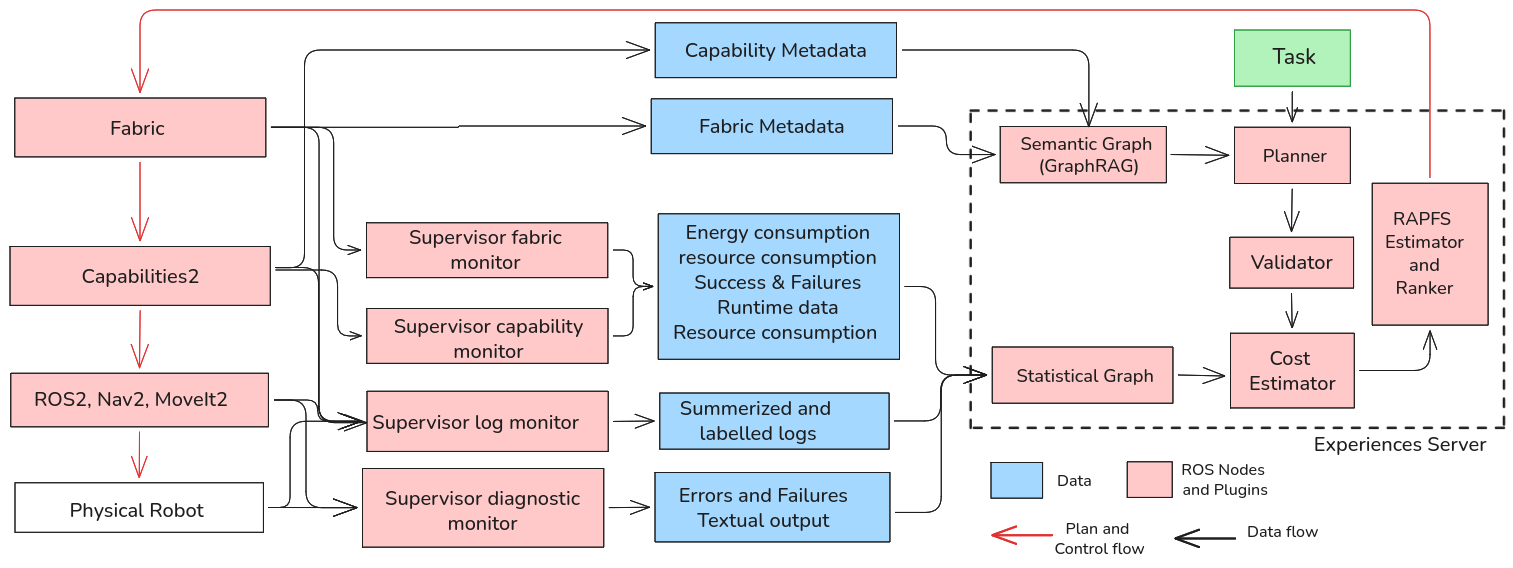
\includegraphics[width=0.8\textwidth]{figures/experience_architecture.png}
    \caption{Architecture of the Experience and Supervisor system.}
    \label{fig:experience_architecture}
\end{figure*}

We run 5 generative tasks related to manipulation in a Physical Techman TM12s robot as shown in Figure \ref{fig:experiment_setup}. We utilise a custom two-finger gripper for the manipulation tasks and a Realsense camera for perception. Anygrasp \cite{fang2023anygrasp} framework is used for grasp pose detection and Ultralytics Yolo26 \cite{jocher2026ultralyticsyolo26unifiedrealtime} is used for object detection. All of these components are integrated into the ROS2 ecosystem to facilitate seamless operation and data collection for the Experience and Supervisor system. All the ROS2 nodes run on a local workstation with an Intel Xeon W3245 processor with 192GB RAM and RTX 3090 with 24GB VRAM.

\begin{figure}
    \centering
        \begin{minipage}[t]{0.30\linewidth}
            \centering
            \includegraphics[width=\linewidth]{figures/experiment_setup.jpg}
        \end{minipage}
        \hfill
        \begin{minipage}[t]{0.58\linewidth}
            \centering
            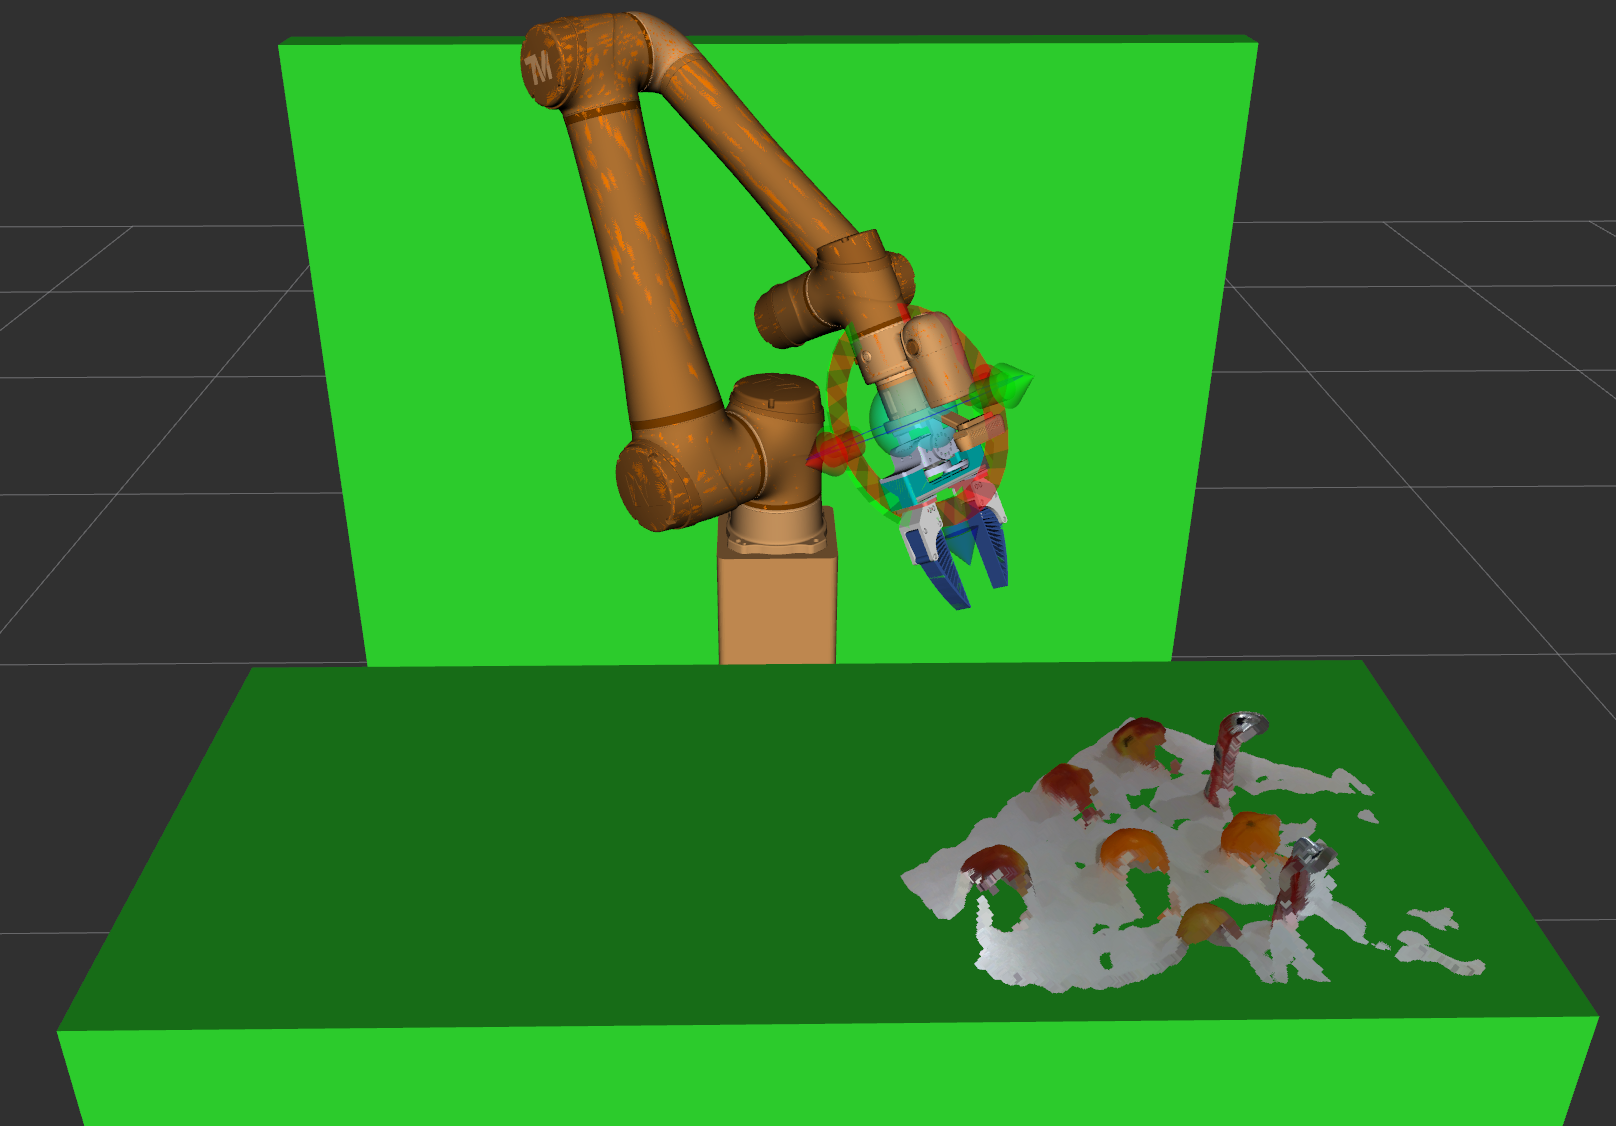
\includegraphics[width=\linewidth]{figures/experiment_setup_moveit.png}
        \end{minipage}
        \caption{Experimental setup with the Physical Techman TM12s robot and the MoveIt planning view.}
    \label{fig:experiment_setup}
\end{figure}

The vision and manipulation tasks used for evaluation are as follows:

\begin{enumerate}
    \item Moving the robot to a system-level predefined pose. 
    \item Moving the robot through a series of predefined poses.
    \item Counting the number of objects in the scene.
    \item Moving the coke cans in the scene to the drop locations.
    \item Moving one of the oranges to the drop location.
\end{enumerate}

These tasks are evaluated under 3 conditions. In the current study, each task is iterated 10 times for direct Fabric generation, and 5 times for each Experience-enabled condition. The evaluation conditions are:

\begin{enumerate}
    \item Fabric for direct plan generation.
    \item Fabric and Experience with Experience initialised from capability semantics but without prior empirical execution evidence.
    \item Fabric and Experience with Experience containing both semantic information and prior empirical run evidence.
\end{enumerate}

In the second evaluation condition, Experience begins with capability semantics and acquires empirical evidence only as tasks are executed during the experiment. In the third condition, Experience is seeded with empirical evidence collected from prior non-generative executions and continues to update that evidence online during evaluation across tasks. This distinction allows us to separate two questions: whether semantic pre-structuring alone improves plan assessment, and whether additional empirical evidence further improves the quality of candidate selection.

To emulate worst-case scenarios, we use a non-fine-tuned version of AnyGrasp, which has not been specifically adapted to the objects or tasks in our evaluation. Also, we disable the functionality of some of the Capabilities to emulate a degraded operational environment. This helps us understand how Experience performs under suboptimal conditions and whether it can still effectively guide plan selection despite incomplete or imperfect information.

As shown in Figure \ref{fig:expected_scores_comparison}, predicted success generally increases and uncertainty tends to decrease as Experience accumulates more evidence. Table \ref{tab:evaluation_results} connects those internal score and reasoning trends to the real robot outcomes. The main pattern is that semantic pre-structuring already stabilises reasoning and improves the easier tasks, while adding prior empirical run evidence produces the best alignment between internal assessment and observed execution, especially for the repeated manipulation case in Task 4. Fault burden was present in some iterations, but the adaptive nature of Experience reduced its downstream effect on plan selection over time. Time, resource utilisation, and energy consumption were not measured here because the study used a limited task set on a stationary manipulator setup.

\begin{figure*}[tb]
    \centering
    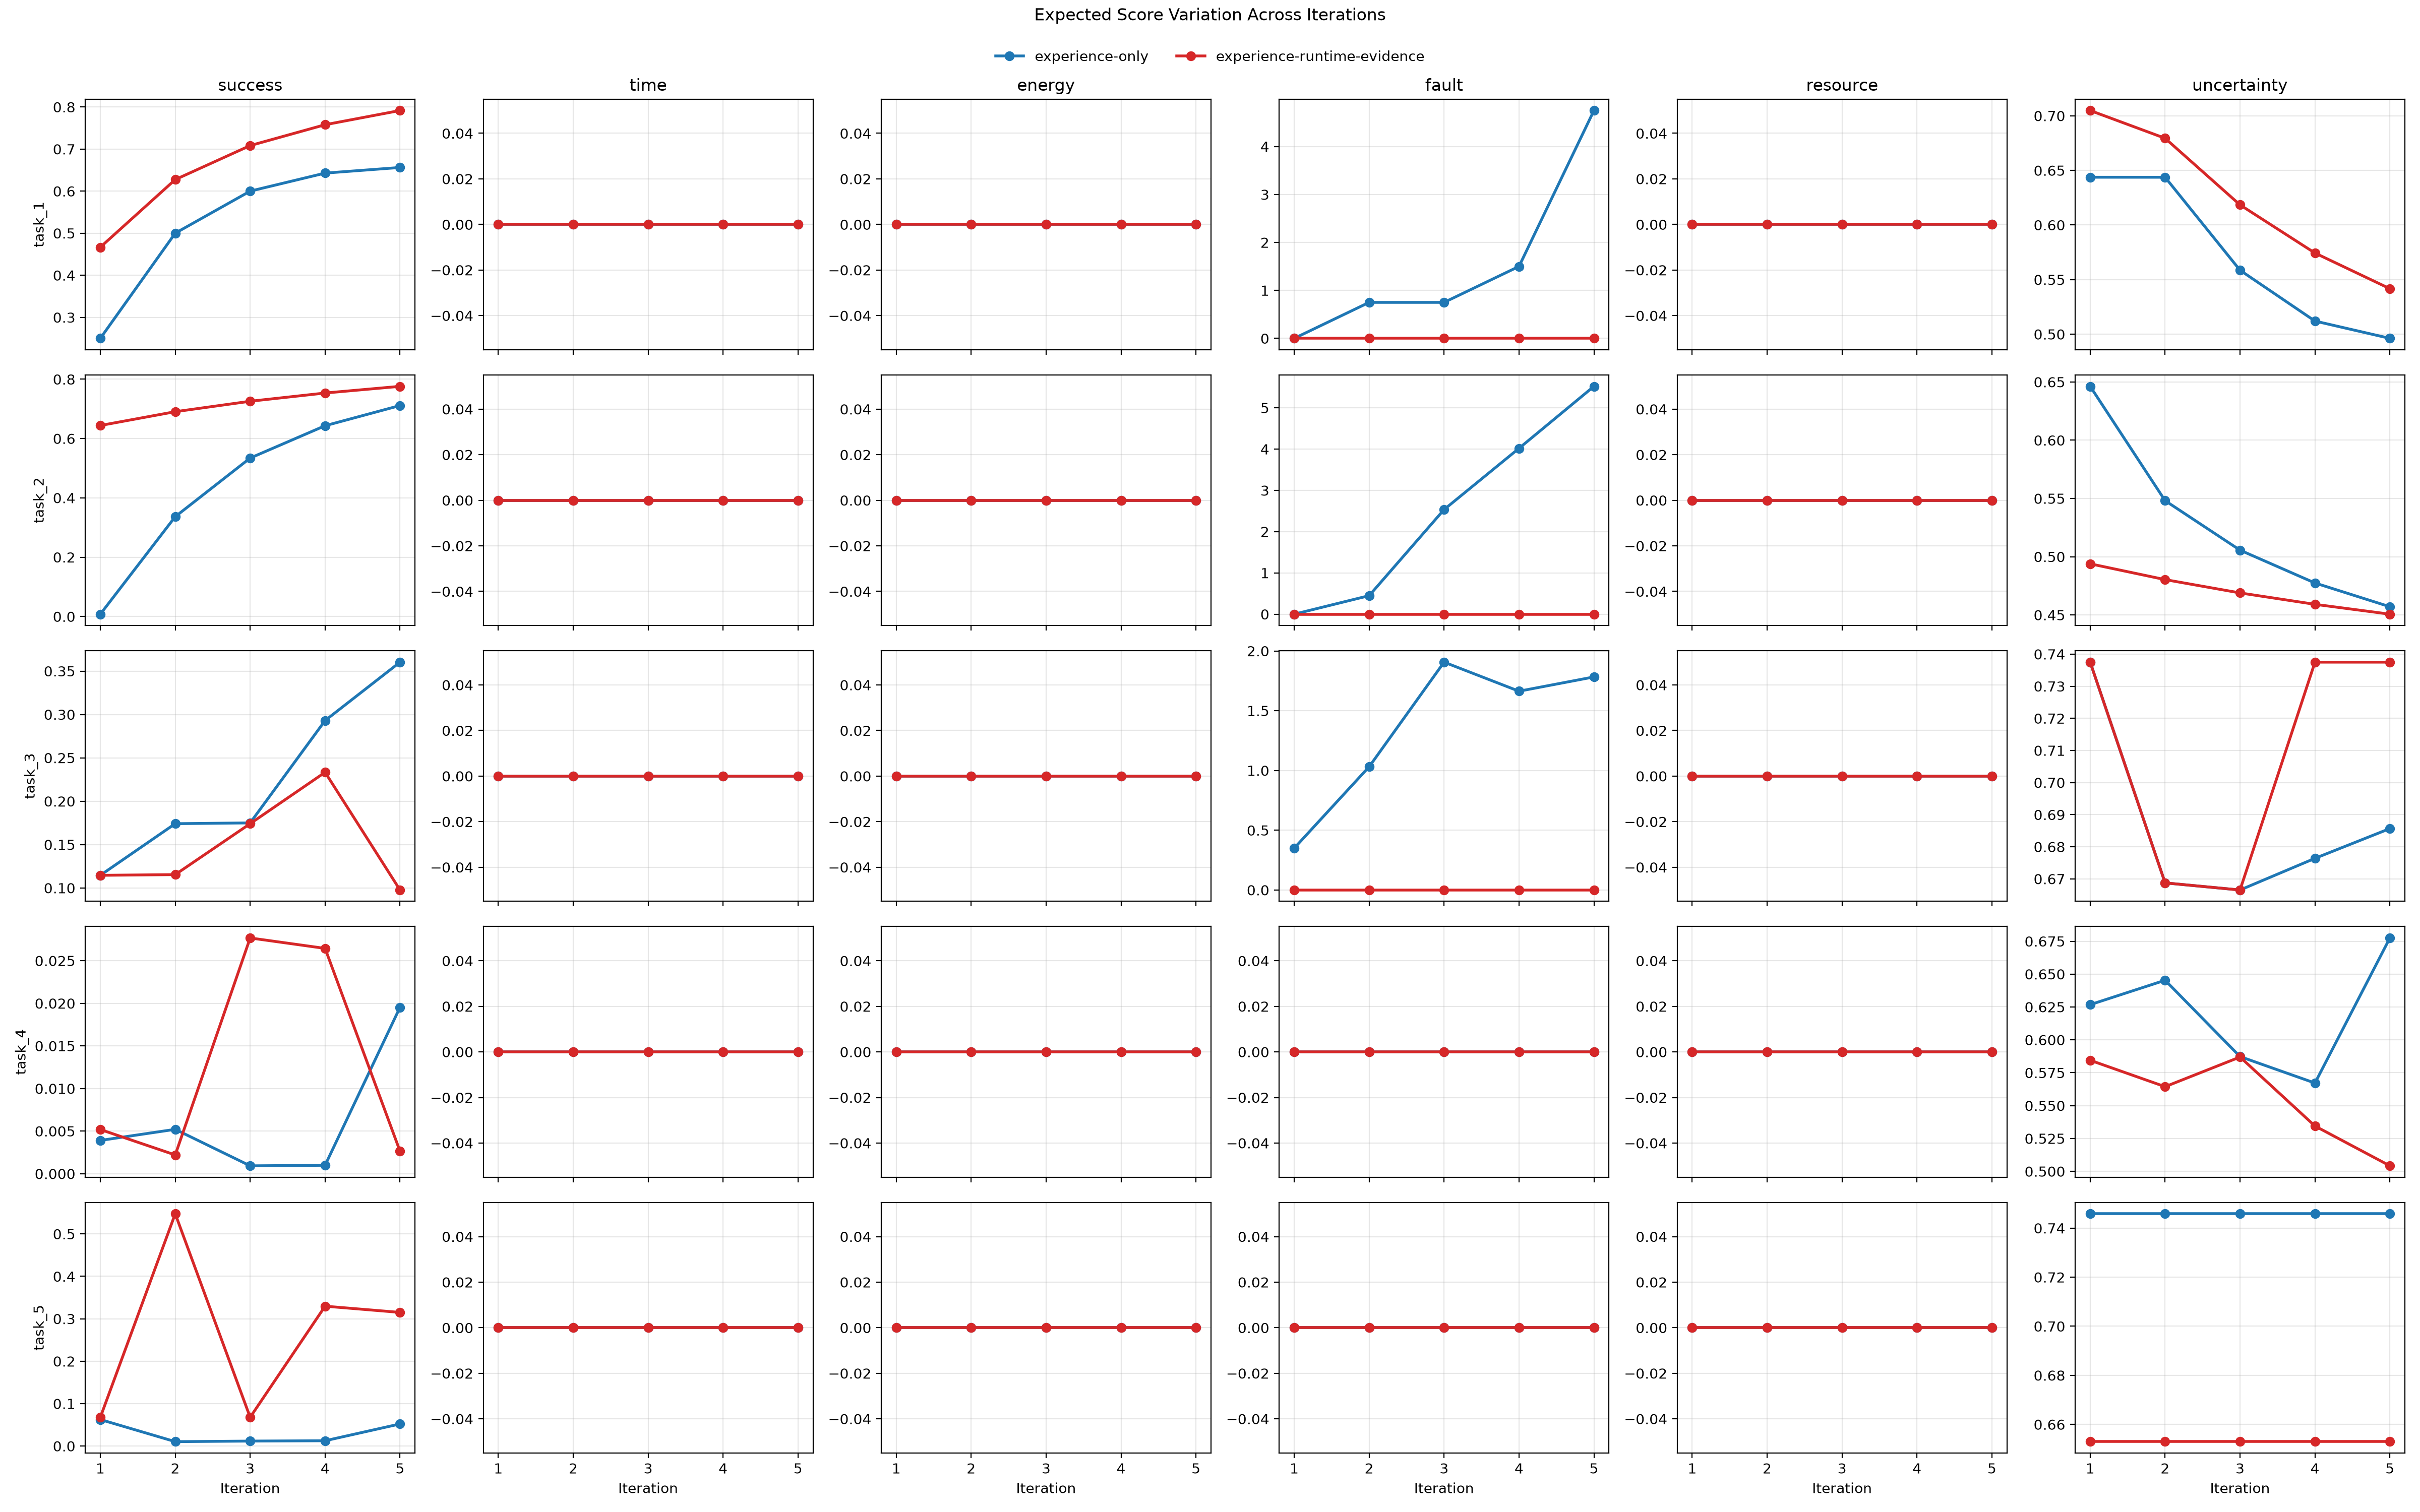
\includegraphics[width=0.9\textwidth]{figures/expected_scores_comparison.png}
    \caption{RAPFS scores component variation across different evaluation conditions.}
    \label{fig:expected_scores_comparison}
\end{figure*}

\begin{table*}[tb]
    \centering
    \caption{Linked summary of internal reasoning trends and real-world task outcomes across evaluation conditions.}
    \label{tab:evaluation_results}
    \footnotesize
    \setlength{\tabcolsep}{4pt}
    \begin{tabular}{@{}>{\raggedright\arraybackslash}p{0.15\textwidth} >{\raggedright\arraybackslash}p{0.26\textwidth} >{\raggedright\arraybackslash}p{0.22\textwidth} >{\raggedright\arraybackslash}p{0.18\textwidth}@{}}
        \toprule
        Approach & Internal reasoning trend & Real-world task results & What this shows \\
        \midrule
        Direct plan generation (Fabric only) & No separate evidence-aware assessment layer is applied before execution, so plan choice depends directly on the generated XML and its immediate semantic plausibility rather than accumulated execution evidence. & Task 1 succeeds in 10/10 runs, Task 2 in 4/10 runs, and Tasks 3--5 fail in all 10 runs with mixed failure causes including wrong XML parameters, wrong control-mode choice, wrong capability choice, and one broken capability case. & Direct generation is sufficient for the simplest task, but it is brittle once the task requires stronger capability selection and execution grounding. \\
        \midrule
        Experience with semantic information only & Internal reasoning converges quickly toward more stable, parser-safe sequential plans. For Tasks 1--4 it reduces exploratory structure over iterations, while Task 5 shows a larger rewrite toward a fully Cartesian manipulation strategy. & Tasks 1 and 2 succeed in 5/5 runs, Task 4 reaches partial success in 2/5 runs, and Tasks 3 and 5 still fail in 5/5 runs. Task 5 failures remain dominated by wrong capability selection. & Semantic structuring alone improves consistency and removes several easy planning errors, but without prior run evidence it still struggles to disambiguate harder manipulation choices. \\
        \midrule
        Experience with semantic + empirical information & Internal reasoning is the most stable and evidence-backed of the three settings. It converges earlier, preserves validated execution patterns, and reduces structural experimentation across iterations. & Tasks 1 and 2 succeed in 5/5 runs, Task 4 reaches partial success in 4/5 runs, Task 3 still fails in 5/5 runs, and Task 5 also fails in 5/5 runs but shifts from capability-selection errors to a consistent XML/configuration error. & This is the strongest overall approach in the current study. Prior run evidence does not solve every hard task, but it improves reasoning-execution alignment and materially improves repeated manipulation performance. \\
        \bottomrule
    \end{tabular}
\end{table*}

The logs, evaluation results and detailed analysis can be found at https://anonymous.4open.science/r/experience-2027-3F4C

\section{Conclusion}

This paper presented \textit{Experience}, an evidence-aware pre-execution assessment layer for generative behaviour-based robot planning. Rather than treating semantically valid plans as equally executable, Experience combines semantic task-behaviour structure with empirical runtime evidence and ranks candidate execution graphs using RAPFS before dispatch. In the current ROS2 implementation, this links Capabilities2 metadata, Fabric-generated candidates, Supervisor runtime feedback, graph-based retrieval, and explainable score-oriented interfaces into one planning loop.

The experimental results show that this additional assessment layer improves the alignment between the robot's internal reasoning and observed execution. Semantic pre-structuring alone already stabilised plan selection and improved the easier tasks, while adding prior empirical run evidence produced the strongest overall behaviour, including more consistent reasoning and better partial performance on the harder repeated manipulation task. At the same time, the remaining failures on Tasks 3 and 5 show that evidence-aware ranking does not by itself resolve all capability-selection, configuration, or perception limitations. The next stage of this work is therefore to extend the evidence model with richer resource and execution signals, evaluate more diverse tasks, and study how the scoring model can be calibrated from larger volumes of runtime feedback.

\bibliographystyle{ieeetr}
\bibliography{references}

\end{document}
